% Created by tikzDevice version 0.12.6 on 2026-07-09 15:42:26
% !TEX encoding = UTF-8 Unicode
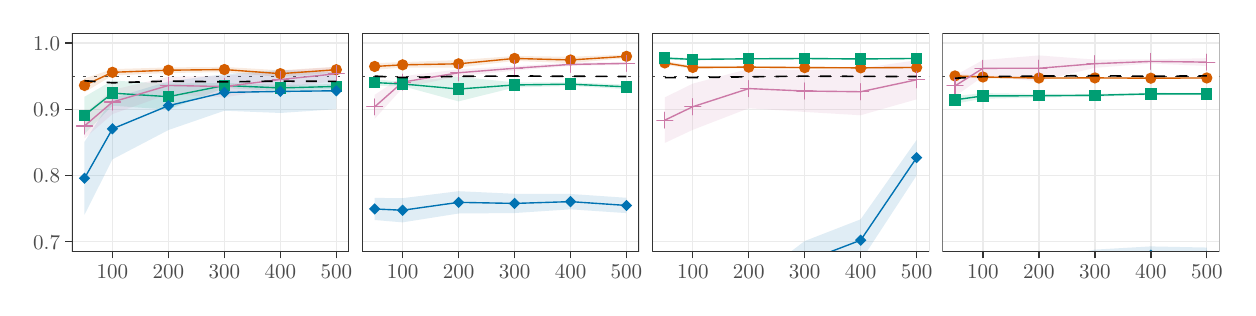
\begin{tikzpicture}[x=1pt,y=1pt]
\definecolor{fillColor}{RGB}{255,255,255}
\path[use as bounding box,fill=fillColor,fill opacity=0.00] (0,0) rectangle (433.62, 93.95);
\begin{scope}
\path[clip] (  0.00,  0.00) rectangle (433.62, 93.95);
\definecolor{drawColor}{RGB}{255,255,255}
\definecolor{fillColor}{RGB}{255,255,255}

\path[draw=drawColor,line width= 0.5pt,line join=round,line cap=round,fill=fillColor] ( -0.00,  0.00) rectangle (433.62, 93.95);
\end{scope}
\begin{scope}
\path[clip] ( 15.98, 12.99) rectangle (116.08, 91.95);
\definecolor{fillColor}{RGB}{255,255,255}

\path[fill=fillColor] ( 15.98, 12.99) rectangle (116.08, 91.95);
\definecolor{drawColor}{gray}{0.92}

\path[draw=drawColor,line width= 0.5pt,line join=round] ( 15.98, 16.58) --
	(116.08, 16.58);

\path[draw=drawColor,line width= 0.5pt,line join=round] ( 15.98, 40.50) --
	(116.08, 40.50);

\path[draw=drawColor,line width= 0.5pt,line join=round] ( 15.98, 64.43) --
	(116.08, 64.43);

\path[draw=drawColor,line width= 0.5pt,line join=round] ( 15.98, 88.36) --
	(116.08, 88.36);

\path[draw=drawColor,line width= 0.5pt,line join=round] ( 30.64, 12.99) --
	( 30.64, 91.95);

\path[draw=drawColor,line width= 0.5pt,line join=round] ( 50.87, 12.99) --
	( 50.87, 91.95);

\path[draw=drawColor,line width= 0.5pt,line join=round] ( 71.09, 12.99) --
	( 71.09, 91.95);

\path[draw=drawColor,line width= 0.5pt,line join=round] ( 91.31, 12.99) --
	( 91.31, 91.95);

\path[draw=drawColor,line width= 0.5pt,line join=round] (111.53, 12.99) --
	(111.53, 91.95);
\definecolor{drawColor}{gray}{0.30}

\path[draw=drawColor,line width= 0.4pt,dash pattern=on 1pt off 3pt ,line join=round] ( 15.98, 76.40) -- (116.08, 76.40);
\definecolor{fillColor}{RGB}{213,94,0}

\path[fill=fillColor,fill opacity=0.12] ( 20.53, 75.60) --
	( 30.64, 78.97) --
	( 50.87, 79.59) --
	( 71.09, 79.77) --
	( 91.31, 78.56) --
	(111.53, 79.80) --
	(111.53, 77.72) --
	( 91.31, 76.09) --
	( 71.09, 77.87) --
	( 50.87, 77.57) --
	( 30.64, 76.68) --
	( 20.53, 70.58) --
	cycle;

\path[] ( 20.53, 75.60) --
	( 30.64, 78.97) --
	( 50.87, 79.59) --
	( 71.09, 79.77) --
	( 91.31, 78.56) --
	(111.53, 79.80);

\path[] (111.53, 77.72) --
	( 91.31, 76.09) --
	( 71.09, 77.87) --
	( 50.87, 77.57) --
	( 30.64, 76.68) --
	( 20.53, 70.58);
\definecolor{fillColor}{RGB}{0,158,115}

\path[fill=fillColor,fill opacity=0.12] ( 20.53, 68.99) --
	( 30.64, 74.85) --
	( 50.87, 73.68) --
	( 71.09, 73.98) --
	( 91.31, 73.32) --
	(111.53, 73.56) --
	(111.53, 71.85) --
	( 91.31, 71.03) --
	( 71.09, 72.15) --
	( 50.87, 64.34) --
	( 30.64, 65.75) --
	( 20.53, 55.57) --
	cycle;

\path[] ( 20.53, 68.99) --
	( 30.64, 74.85) --
	( 50.87, 73.68) --
	( 71.09, 73.98) --
	( 91.31, 73.32) --
	(111.53, 73.56);

\path[] (111.53, 71.85) --
	( 91.31, 71.03) --
	( 71.09, 72.15) --
	( 50.87, 64.34) --
	( 30.64, 65.75) --
	( 20.53, 55.57);
\definecolor{fillColor}{RGB}{0,114,178}

\path[fill=fillColor,fill opacity=0.12] ( 20.53, 52.70) --
	( 30.64, 68.43) --
	( 50.87, 74.55) --
	( 71.09, 77.15) --
	( 91.31, 78.70) --
	(111.53, 77.81) --
	(111.53, 64.49) --
	( 91.31, 63.13) --
	( 71.09, 63.94) --
	( 50.87, 56.97) --
	( 30.64, 46.38) --
	( 20.53, 26.35) --
	cycle;

\path[] ( 20.53, 52.70) --
	( 30.64, 68.43) --
	( 50.87, 74.55) --
	( 71.09, 77.15) --
	( 91.31, 78.70) --
	(111.53, 77.81);

\path[] (111.53, 64.49) --
	( 91.31, 63.13) --
	( 71.09, 63.94) --
	( 50.87, 56.97) --
	( 30.64, 46.38) --
	( 20.53, 26.35);
\definecolor{fillColor}{RGB}{204,121,167}

\path[fill=fillColor,fill opacity=0.12] ( 20.53, 62.93) --
	( 30.64, 71.45) --
	( 50.87, 76.23) --
	( 71.09, 76.58) --
	( 91.31, 78.35) --
	(111.53, 79.83) --
	(111.53, 74.75) --
	( 91.31, 72.07) --
	( 71.09, 68.77) --
	( 50.87, 69.91) --
	( 30.64, 62.72) --
	( 20.53, 53.93) --
	cycle;

\path[] ( 20.53, 62.93) --
	( 30.64, 71.45) --
	( 50.87, 76.23) --
	( 71.09, 76.58) --
	( 91.31, 78.35) --
	(111.53, 79.83);

\path[] (111.53, 74.75) --
	( 91.31, 72.07) --
	( 71.09, 68.77) --
	( 50.87, 69.91) --
	( 30.64, 62.72) --
	( 20.53, 53.93);
\definecolor{drawColor}{RGB}{213,94,0}

\path[draw=drawColor,line width= 0.5pt,line join=round] ( 20.53, 73.09) --
	( 30.64, 77.82) --
	( 50.87, 78.58) --
	( 71.09, 78.82) --
	( 91.31, 77.33) --
	(111.53, 78.76);
\definecolor{drawColor}{RGB}{0,158,115}

\path[draw=drawColor,line width= 0.5pt,line join=round] ( 20.53, 62.28) --
	( 30.64, 70.30) --
	( 50.87, 69.01) --
	( 71.09, 73.06) --
	( 91.31, 72.17) --
	(111.53, 72.71);
\definecolor{drawColor}{RGB}{0,114,178}

\path[draw=drawColor,line width= 0.5pt,line join=round] ( 20.53, 39.53) --
	( 30.64, 57.40) --
	( 50.87, 65.76) --
	( 71.09, 70.55) --
	( 91.31, 70.91) --
	(111.53, 71.15);
\definecolor{drawColor}{RGB}{204,121,167}

\path[draw=drawColor,line width= 0.5pt,line join=round] ( 20.53, 58.43) --
	( 30.64, 67.09) --
	( 50.87, 73.07) --
	( 71.09, 72.68) --
	( 91.31, 75.21) --
	(111.53, 77.29);
\definecolor{fillColor}{RGB}{213,94,0}

\path[fill=fillColor] ( 20.53, 73.09) circle (  2.05);

\path[draw=drawColor,line width= 0.4pt,line join=round,line cap=round] ( 17.63, 58.43) -- ( 23.43, 58.43);

\path[draw=drawColor,line width= 0.4pt,line join=round,line cap=round] ( 20.53, 55.53) -- ( 20.53, 61.33);
\definecolor{fillColor}{RGB}{0,158,115}

\path[fill=fillColor] ( 18.48, 60.23) --
	( 22.58, 60.23) --
	( 22.58, 64.33) --
	( 18.48, 64.33) --
	cycle;
\definecolor{fillColor}{RGB}{0,114,178}

\path[fill=fillColor] ( 18.48, 39.53) --
	( 20.53, 41.58) --
	( 22.58, 39.53) --
	( 20.53, 37.47) --
	cycle;
\definecolor{fillColor}{RGB}{213,94,0}

\path[fill=fillColor] ( 30.64, 77.82) circle (  2.05);

\path[draw=drawColor,line width= 0.4pt,line join=round,line cap=round] ( 27.74, 67.09) -- ( 33.55, 67.09);

\path[draw=drawColor,line width= 0.4pt,line join=round,line cap=round] ( 30.64, 64.18) -- ( 30.64, 69.99);
\definecolor{fillColor}{RGB}{0,158,115}

\path[fill=fillColor] ( 28.59, 68.25) --
	( 32.70, 68.25) --
	( 32.70, 72.35) --
	( 28.59, 72.35) --
	cycle;
\definecolor{fillColor}{RGB}{0,114,178}

\path[fill=fillColor] ( 28.59, 57.40) --
	( 30.64, 59.46) --
	( 32.70, 57.40) --
	( 30.64, 55.35) --
	cycle;
\definecolor{fillColor}{RGB}{213,94,0}

\path[fill=fillColor] ( 50.87, 78.58) circle (  2.05);

\path[draw=drawColor,line width= 0.4pt,line join=round,line cap=round] ( 47.96, 73.07) -- ( 53.77, 73.07);

\path[draw=drawColor,line width= 0.4pt,line join=round,line cap=round] ( 50.87, 70.17) -- ( 50.87, 75.97);
\definecolor{fillColor}{RGB}{0,158,115}

\path[fill=fillColor] ( 48.81, 66.96) --
	( 52.92, 66.96) --
	( 52.92, 71.06) --
	( 48.81, 71.06) --
	cycle;
\definecolor{fillColor}{RGB}{0,114,178}

\path[fill=fillColor] ( 48.81, 65.76) --
	( 50.87, 67.81) --
	( 52.92, 65.76) --
	( 50.87, 63.71) --
	cycle;
\definecolor{fillColor}{RGB}{213,94,0}

\path[fill=fillColor] ( 71.09, 78.82) circle (  2.05);

\path[draw=drawColor,line width= 0.4pt,line join=round,line cap=round] ( 68.19, 72.68) -- ( 73.99, 72.68);

\path[draw=drawColor,line width= 0.4pt,line join=round,line cap=round] ( 71.09, 69.78) -- ( 71.09, 75.58);
\definecolor{fillColor}{RGB}{0,158,115}

\path[fill=fillColor] ( 69.04, 71.01) --
	( 73.14, 71.01) --
	( 73.14, 75.11) --
	( 69.04, 75.11) --
	cycle;
\definecolor{fillColor}{RGB}{0,114,178}

\path[fill=fillColor] ( 69.04, 70.55) --
	( 71.09, 72.60) --
	( 73.14, 70.55) --
	( 71.09, 68.50) --
	cycle;
\definecolor{fillColor}{RGB}{213,94,0}

\path[fill=fillColor] ( 91.31, 77.33) circle (  2.05);

\path[draw=drawColor,line width= 0.4pt,line join=round,line cap=round] ( 88.41, 75.21) -- ( 94.21, 75.21);

\path[draw=drawColor,line width= 0.4pt,line join=round,line cap=round] ( 91.31, 72.31) -- ( 91.31, 78.11);
\definecolor{fillColor}{RGB}{0,158,115}

\path[fill=fillColor] ( 89.26, 70.12) --
	( 93.36, 70.12) --
	( 93.36, 74.23) --
	( 89.26, 74.23) --
	cycle;
\definecolor{fillColor}{RGB}{0,114,178}

\path[fill=fillColor] ( 89.26, 70.91) --
	( 91.31, 72.96) --
	( 93.36, 70.91) --
	( 91.31, 68.86) --
	cycle;
\definecolor{fillColor}{RGB}{213,94,0}

\path[fill=fillColor] (111.53, 78.76) circle (  2.05);

\path[draw=drawColor,line width= 0.4pt,line join=round,line cap=round] (108.63, 77.29) -- (114.43, 77.29);

\path[draw=drawColor,line width= 0.4pt,line join=round,line cap=round] (111.53, 74.39) -- (111.53, 80.19);
\definecolor{fillColor}{RGB}{0,158,115}

\path[fill=fillColor] (109.48, 70.65) --
	(113.58, 70.65) --
	(113.58, 74.76) --
	(109.48, 74.76) --
	cycle;
\definecolor{fillColor}{RGB}{0,114,178}

\path[fill=fillColor] (109.48, 71.15) --
	(111.53, 73.20) --
	(113.58, 71.15) --
	(111.53, 69.10) --
	cycle;
\definecolor{drawColor}{RGB}{0,0,0}

\path[draw=drawColor,line width= 0.6pt,dash pattern=on 4pt off 4pt ,line join=round] ( 20.53, 74.77) --
	( 30.64, 74.04) --
	( 50.87, 74.65) --
	( 71.09, 74.36) --
	( 91.31, 74.64) --
	(111.53, 74.53);
\definecolor{drawColor}{gray}{0.20}

\path[draw=drawColor,line width= 0.5pt,line join=round,line cap=round] ( 15.98, 12.99) rectangle (116.08, 91.95);
\end{scope}
\begin{scope}
\path[clip] (120.83, 12.99) rectangle (220.93, 91.95);
\definecolor{fillColor}{RGB}{255,255,255}

\path[fill=fillColor] (120.83, 12.99) rectangle (220.93, 91.95);
\definecolor{drawColor}{gray}{0.92}

\path[draw=drawColor,line width= 0.5pt,line join=round] (120.83, 16.58) --
	(220.93, 16.58);

\path[draw=drawColor,line width= 0.5pt,line join=round] (120.83, 40.50) --
	(220.93, 40.50);

\path[draw=drawColor,line width= 0.5pt,line join=round] (120.83, 64.43) --
	(220.93, 64.43);

\path[draw=drawColor,line width= 0.5pt,line join=round] (120.83, 88.36) --
	(220.93, 88.36);

\path[draw=drawColor,line width= 0.5pt,line join=round] (135.49, 12.99) --
	(135.49, 91.95);

\path[draw=drawColor,line width= 0.5pt,line join=round] (155.71, 12.99) --
	(155.71, 91.95);

\path[draw=drawColor,line width= 0.5pt,line join=round] (175.93, 12.99) --
	(175.93, 91.95);

\path[draw=drawColor,line width= 0.5pt,line join=round] (196.16, 12.99) --
	(196.16, 91.95);

\path[draw=drawColor,line width= 0.5pt,line join=round] (216.38, 12.99) --
	(216.38, 91.95);
\definecolor{drawColor}{gray}{0.30}

\path[draw=drawColor,line width= 0.4pt,dash pattern=on 1pt off 3pt ,line join=round] (120.83, 76.40) -- (220.93, 76.40);
\definecolor{fillColor}{RGB}{213,94,0}

\path[fill=fillColor,fill opacity=0.12] (125.38, 81.12) --
	(135.49, 81.52) --
	(155.71, 82.22) --
	(175.93, 83.72) --
	(196.16, 83.43) --
	(216.38, 84.24) --
	(216.38, 82.94) --
	(196.16, 81.13) --
	(175.93, 81.94) --
	(155.71, 79.56) --
	(135.49, 79.52) --
	(125.38, 78.74) --
	cycle;

\path[] (125.38, 81.12) --
	(135.49, 81.52) --
	(155.71, 82.22) --
	(175.93, 83.72) --
	(196.16, 83.43) --
	(216.38, 84.24);

\path[] (216.38, 82.94) --
	(196.16, 81.13) --
	(175.93, 81.94) --
	(155.71, 79.56) --
	(135.49, 79.52) --
	(125.38, 78.74);
\definecolor{fillColor}{RGB}{0,158,115}

\path[fill=fillColor,fill opacity=0.12] (125.38, 75.29) --
	(135.49, 74.40) --
	(155.71, 76.24) --
	(175.93, 74.17) --
	(196.16, 74.19) --
	(216.38, 73.40) --
	(216.38, 71.74) --
	(196.16, 72.89) --
	(175.93, 72.34) --
	(155.71, 67.32) --
	(135.49, 72.82) --
	(125.38, 72.90) --
	cycle;

\path[] (125.38, 75.29) --
	(135.49, 74.40) --
	(155.71, 76.24) --
	(175.93, 74.17) --
	(196.16, 74.19) --
	(216.38, 73.40);

\path[] (216.38, 71.74) --
	(196.16, 72.89) --
	(175.93, 72.34) --
	(155.71, 67.32) --
	(135.49, 72.82) --
	(125.38, 72.90);
\definecolor{fillColor}{RGB}{0,114,178}

\path[fill=fillColor,fill opacity=0.12] (125.38, 32.43) --
	(135.49, 32.35) --
	(155.71, 34.86) --
	(175.93, 33.92) --
	(196.16, 33.86) --
	(216.38, 32.48) --
	(216.38, 26.94) --
	(196.16, 28.31) --
	(175.93, 26.97) --
	(155.71, 26.80) --
	(135.49, 23.60) --
	(125.38, 24.45) --
	cycle;

\path[] (125.38, 32.43) --
	(135.49, 32.35) --
	(155.71, 34.86) --
	(175.93, 33.92) --
	(196.16, 33.86) --
	(216.38, 32.48);

\path[] (216.38, 26.94) --
	(196.16, 28.31) --
	(175.93, 26.97) --
	(155.71, 26.80) --
	(135.49, 23.60) --
	(125.38, 24.45);
\definecolor{fillColor}{RGB}{204,121,167}

\path[fill=fillColor,fill opacity=0.12] (125.38, 69.67) --
	(135.49, 76.38) --
	(155.71, 78.89) --
	(175.93, 80.11) --
	(196.16, 81.25) --
	(216.38, 81.50) --
	(216.38, 80.57) --
	(196.16, 80.10) --
	(175.93, 78.43) --
	(155.71, 76.43) --
	(135.49, 72.17) --
	(125.38, 61.00) --
	cycle;

\path[] (125.38, 69.67) --
	(135.49, 76.38) --
	(155.71, 78.89) --
	(175.93, 80.11) --
	(196.16, 81.25) --
	(216.38, 81.50);

\path[] (216.38, 80.57) --
	(196.16, 80.10) --
	(175.93, 78.43) --
	(155.71, 76.43) --
	(135.49, 72.17) --
	(125.38, 61.00);
\definecolor{drawColor}{RGB}{213,94,0}

\path[draw=drawColor,line width= 0.5pt,line join=round] (125.38, 79.93) --
	(135.49, 80.52) --
	(155.71, 80.89) --
	(175.93, 82.83) --
	(196.16, 82.28) --
	(216.38, 83.59);
\definecolor{drawColor}{RGB}{0,158,115}

\path[draw=drawColor,line width= 0.5pt,line join=round] (125.38, 74.10) --
	(135.49, 73.61) --
	(155.71, 71.78) --
	(175.93, 73.25) --
	(196.16, 73.54) --
	(216.38, 72.57);
\definecolor{drawColor}{RGB}{0,114,178}

\path[draw=drawColor,line width= 0.5pt,line join=round] (125.38, 28.44) --
	(135.49, 27.98) --
	(155.71, 30.83) --
	(175.93, 30.44) --
	(196.16, 31.09) --
	(216.38, 29.71);
\definecolor{drawColor}{RGB}{204,121,167}

\path[draw=drawColor,line width= 0.5pt,line join=round] (125.38, 65.34) --
	(135.49, 74.28) --
	(155.71, 77.66) --
	(175.93, 79.27) --
	(196.16, 80.67) --
	(216.38, 81.03);
\definecolor{fillColor}{RGB}{213,94,0}

\path[fill=fillColor] (125.38, 79.93) circle (  2.05);

\path[draw=drawColor,line width= 0.4pt,line join=round,line cap=round] (122.48, 65.34) -- (128.28, 65.34);

\path[draw=drawColor,line width= 0.4pt,line join=round,line cap=round] (125.38, 62.44) -- (125.38, 68.24);
\definecolor{fillColor}{RGB}{0,158,115}

\path[fill=fillColor] (123.33, 72.04) --
	(127.43, 72.04) --
	(127.43, 76.15) --
	(123.33, 76.15) --
	cycle;
\definecolor{fillColor}{RGB}{0,114,178}

\path[fill=fillColor] (123.33, 28.44) --
	(125.38, 30.49) --
	(127.43, 28.44) --
	(125.38, 26.39) --
	cycle;
\definecolor{fillColor}{RGB}{213,94,0}

\path[fill=fillColor] (135.49, 80.52) circle (  2.05);

\path[draw=drawColor,line width= 0.4pt,line join=round,line cap=round] (132.59, 74.28) -- (138.39, 74.28);

\path[draw=drawColor,line width= 0.4pt,line join=round,line cap=round] (135.49, 71.38) -- (135.49, 77.18);
\definecolor{fillColor}{RGB}{0,158,115}

\path[fill=fillColor] (133.44, 71.56) --
	(137.54, 71.56) --
	(137.54, 75.66) --
	(133.44, 75.66) --
	cycle;
\definecolor{fillColor}{RGB}{0,114,178}

\path[fill=fillColor] (133.44, 27.98) --
	(135.49, 30.03) --
	(137.54, 27.98) --
	(135.49, 25.92) --
	cycle;
\definecolor{fillColor}{RGB}{213,94,0}

\path[fill=fillColor] (155.71, 80.89) circle (  2.05);

\path[draw=drawColor,line width= 0.4pt,line join=round,line cap=round] (152.81, 77.66) -- (158.61, 77.66);

\path[draw=drawColor,line width= 0.4pt,line join=round,line cap=round] (155.71, 74.76) -- (155.71, 80.56);
\definecolor{fillColor}{RGB}{0,158,115}

\path[fill=fillColor] (153.66, 69.73) --
	(157.76, 69.73) --
	(157.76, 73.83) --
	(153.66, 73.83) --
	cycle;
\definecolor{fillColor}{RGB}{0,114,178}

\path[fill=fillColor] (153.66, 30.83) --
	(155.71, 32.88) --
	(157.76, 30.83) --
	(155.71, 28.78) --
	cycle;
\definecolor{fillColor}{RGB}{213,94,0}

\path[fill=fillColor] (175.93, 82.83) circle (  2.05);

\path[draw=drawColor,line width= 0.4pt,line join=round,line cap=round] (173.03, 79.27) -- (178.83, 79.27);

\path[draw=drawColor,line width= 0.4pt,line join=round,line cap=round] (175.93, 76.37) -- (175.93, 82.17);
\definecolor{fillColor}{RGB}{0,158,115}

\path[fill=fillColor] (173.88, 71.20) --
	(177.99, 71.20) --
	(177.99, 75.30) --
	(173.88, 75.30) --
	cycle;
\definecolor{fillColor}{RGB}{0,114,178}

\path[fill=fillColor] (173.88, 30.44) --
	(175.93, 32.50) --
	(177.99, 30.44) --
	(175.93, 28.39) --
	cycle;
\definecolor{fillColor}{RGB}{213,94,0}

\path[fill=fillColor] (196.16, 82.28) circle (  2.05);

\path[draw=drawColor,line width= 0.4pt,line join=round,line cap=round] (193.25, 80.67) -- (199.06, 80.67);

\path[draw=drawColor,line width= 0.4pt,line join=round,line cap=round] (196.16, 77.77) -- (196.16, 83.57);
\definecolor{fillColor}{RGB}{0,158,115}

\path[fill=fillColor] (194.10, 71.49) --
	(198.21, 71.49) --
	(198.21, 75.59) --
	(194.10, 75.59) --
	cycle;
\definecolor{fillColor}{RGB}{0,114,178}

\path[fill=fillColor] (194.10, 31.09) --
	(196.16, 33.14) --
	(198.21, 31.09) --
	(196.16, 29.04) --
	cycle;
\definecolor{fillColor}{RGB}{213,94,0}

\path[fill=fillColor] (216.38, 83.59) circle (  2.05);

\path[draw=drawColor,line width= 0.4pt,line join=round,line cap=round] (213.48, 81.03) -- (219.28, 81.03);

\path[draw=drawColor,line width= 0.4pt,line join=round,line cap=round] (216.38, 78.13) -- (216.38, 83.94);
\definecolor{fillColor}{RGB}{0,158,115}

\path[fill=fillColor] (214.33, 70.52) --
	(218.43, 70.52) --
	(218.43, 74.62) --
	(214.33, 74.62) --
	cycle;
\definecolor{fillColor}{RGB}{0,114,178}

\path[fill=fillColor] (214.33, 29.71) --
	(216.38, 31.76) --
	(218.43, 29.71) --
	(216.38, 27.66) --
	cycle;
\definecolor{drawColor}{RGB}{0,0,0}

\path[draw=drawColor,line width= 0.6pt,dash pattern=on 4pt off 4pt ,line join=round] (125.38, 76.43) --
	(135.49, 75.91) --
	(155.71, 76.38) --
	(175.93, 76.49) --
	(196.16, 76.39) --
	(216.38, 76.31);
\definecolor{drawColor}{gray}{0.20}

\path[draw=drawColor,line width= 0.5pt,line join=round,line cap=round] (120.83, 12.99) rectangle (220.93, 91.95);
\end{scope}
\begin{scope}
\path[clip] (225.68, 12.99) rectangle (325.77, 91.95);
\definecolor{fillColor}{RGB}{255,255,255}

\path[fill=fillColor] (225.68, 12.99) rectangle (325.77, 91.95);
\definecolor{drawColor}{gray}{0.92}

\path[draw=drawColor,line width= 0.5pt,line join=round] (225.68, 16.58) --
	(325.77, 16.58);

\path[draw=drawColor,line width= 0.5pt,line join=round] (225.68, 40.50) --
	(325.77, 40.50);

\path[draw=drawColor,line width= 0.5pt,line join=round] (225.68, 64.43) --
	(325.77, 64.43);

\path[draw=drawColor,line width= 0.5pt,line join=round] (225.68, 88.36) --
	(325.77, 88.36);

\path[draw=drawColor,line width= 0.5pt,line join=round] (240.34, 12.99) --
	(240.34, 91.95);

\path[draw=drawColor,line width= 0.5pt,line join=round] (260.56, 12.99) --
	(260.56, 91.95);

\path[draw=drawColor,line width= 0.5pt,line join=round] (280.78, 12.99) --
	(280.78, 91.95);

\path[draw=drawColor,line width= 0.5pt,line join=round] (301.00, 12.99) --
	(301.00, 91.95);

\path[draw=drawColor,line width= 0.5pt,line join=round] (321.22, 12.99) --
	(321.22, 91.95);
\definecolor{drawColor}{gray}{0.30}

\path[draw=drawColor,line width= 0.4pt,dash pattern=on 1pt off 3pt ,line join=round] (225.68, 76.40) -- (325.77, 76.40);
\definecolor{fillColor}{RGB}{213,94,0}

\path[fill=fillColor,fill opacity=0.12] (230.23, 81.95) --
	(240.34, 80.15) --
	(260.56, 80.09) --
	(280.78, 79.88) --
	(301.00, 79.79) --
	(321.22, 79.87) --
	(321.22, 79.28) --
	(301.00, 79.07) --
	(280.78, 79.16) --
	(260.56, 79.29) --
	(240.34, 79.03) --
	(230.23, 80.48) --
	cycle;

\path[] (230.23, 81.95) --
	(240.34, 80.15) --
	(260.56, 80.09) --
	(280.78, 79.88) --
	(301.00, 79.79) --
	(321.22, 79.87);

\path[] (321.22, 79.28) --
	(301.00, 79.07) --
	(280.78, 79.16) --
	(260.56, 79.29) --
	(240.34, 79.03) --
	(230.23, 80.48);
\definecolor{fillColor}{RGB}{0,158,115}

\path[fill=fillColor,fill opacity=0.12] (230.23, 83.47) --
	(240.34, 82.86) --
	(260.56, 83.00) --
	(280.78, 83.08) --
	(301.00, 82.89) --
	(321.22, 83.08) --
	(321.22, 82.57) --
	(301.00, 82.39) --
	(280.78, 82.54) --
	(260.56, 82.40) --
	(240.34, 82.11) --
	(230.23, 82.44) --
	cycle;

\path[] (230.23, 83.47) --
	(240.34, 82.86) --
	(260.56, 83.00) --
	(280.78, 83.08) --
	(301.00, 82.89) --
	(321.22, 83.08);

\path[] (321.22, 82.57) --
	(301.00, 82.39) --
	(280.78, 82.54) --
	(260.56, 82.40) --
	(240.34, 82.11) --
	(230.23, 82.44);
\definecolor{fillColor}{RGB}{0,114,178}

\path[fill=fillColor,fill opacity=0.12] (230.23,  0.26) --
	(240.34, -7.03) --
	(260.56,  1.51) --
	(280.78, 16.85) --
	(301.00, 24.70) --
	(321.22, 53.36) --
	(321.22, 40.57) --
	(301.00,  9.60) --
	(280.78,  2.00) --
	(260.56,-10.93) --
	(240.34,-18.89) --
	(230.23,-13.29) --
	cycle;

\path[] (230.23,  0.26) --
	(240.34, -7.03) --
	(260.56,  1.51) --
	(280.78, 16.85) --
	(301.00, 24.70) --
	(321.22, 53.36);

\path[] (321.22, 40.57) --
	(301.00,  9.60) --
	(280.78,  2.00) --
	(260.56,-10.93) --
	(240.34,-18.89) --
	(230.23,-13.29);
\definecolor{fillColor}{RGB}{204,121,167}

\path[fill=fillColor,fill opacity=0.12] (230.23, 68.76) --
	(240.34, 73.73) --
	(260.56, 79.06) --
	(280.78, 78.61) --
	(301.00, 79.29) --
	(321.22, 82.17) --
	(321.22, 68.07) --
	(301.00, 62.30) --
	(280.78, 63.50) --
	(260.56, 64.83) --
	(240.34, 57.04) --
	(230.23, 52.30) --
	cycle;

\path[] (230.23, 68.76) --
	(240.34, 73.73) --
	(260.56, 79.06) --
	(280.78, 78.61) --
	(301.00, 79.29) --
	(321.22, 82.17);

\path[] (321.22, 68.07) --
	(301.00, 62.30) --
	(280.78, 63.50) --
	(260.56, 64.83) --
	(240.34, 57.04) --
	(230.23, 52.30);
\definecolor{drawColor}{RGB}{213,94,0}

\path[draw=drawColor,line width= 0.5pt,line join=round] (230.23, 81.21) --
	(240.34, 79.59) --
	(260.56, 79.69) --
	(280.78, 79.52) --
	(301.00, 79.43) --
	(321.22, 79.57);
\definecolor{drawColor}{RGB}{0,158,115}

\path[draw=drawColor,line width= 0.5pt,line join=round] (230.23, 82.95) --
	(240.34, 82.49) --
	(260.56, 82.70) --
	(280.78, 82.81) --
	(301.00, 82.64) --
	(321.22, 82.83);
\definecolor{drawColor}{RGB}{0,114,178}

\path[draw=drawColor,line width= 0.5pt,line join=round] (230.23, -6.51) --
	(240.34,-12.96) --
	(260.56, -4.71) --
	(280.78,  9.42) --
	(301.00, 17.15) --
	(321.22, 46.97);
\definecolor{drawColor}{RGB}{204,121,167}

\path[draw=drawColor,line width= 0.5pt,line join=round] (230.23, 60.53) --
	(240.34, 65.38) --
	(260.56, 71.94) --
	(280.78, 71.05) --
	(301.00, 70.80) --
	(321.22, 75.12);
\definecolor{fillColor}{RGB}{213,94,0}

\path[fill=fillColor] (230.23, 81.21) circle (  2.05);

\path[draw=drawColor,line width= 0.4pt,line join=round,line cap=round] (227.33, 60.53) -- (233.13, 60.53);

\path[draw=drawColor,line width= 0.4pt,line join=round,line cap=round] (230.23, 57.63) -- (230.23, 63.43);
\definecolor{fillColor}{RGB}{0,158,115}

\path[fill=fillColor] (228.18, 80.90) --
	(232.28, 80.90) --
	(232.28, 85.01) --
	(228.18, 85.01) --
	cycle;
\definecolor{fillColor}{RGB}{0,114,178}

\path[fill=fillColor] (228.18, -6.51) --
	(230.23, -4.46) --
	(232.28, -6.51) --
	(230.23, -8.56) --
	cycle;
\definecolor{fillColor}{RGB}{213,94,0}

\path[fill=fillColor] (240.34, 79.59) circle (  2.05);

\path[draw=drawColor,line width= 0.4pt,line join=round,line cap=round] (237.44, 65.38) -- (243.24, 65.38);

\path[draw=drawColor,line width= 0.4pt,line join=round,line cap=round] (240.34, 62.48) -- (240.34, 68.28);
\definecolor{fillColor}{RGB}{0,158,115}

\path[fill=fillColor] (238.29, 80.44) --
	(242.39, 80.44) --
	(242.39, 84.54) --
	(238.29, 84.54) --
	cycle;
\definecolor{fillColor}{RGB}{0,114,178}

\path[fill=fillColor] (238.29,-12.96) --
	(240.34,-10.91) --
	(242.39,-12.96) --
	(240.34,-15.01) --
	cycle;
\definecolor{fillColor}{RGB}{213,94,0}

\path[fill=fillColor] (260.56, 79.69) circle (  2.05);

\path[draw=drawColor,line width= 0.4pt,line join=round,line cap=round] (257.66, 71.94) -- (263.46, 71.94);

\path[draw=drawColor,line width= 0.4pt,line join=round,line cap=round] (260.56, 69.04) -- (260.56, 74.85);
\definecolor{fillColor}{RGB}{0,158,115}

\path[fill=fillColor] (258.51, 80.65) --
	(262.61, 80.65) --
	(262.61, 84.75) --
	(258.51, 84.75) --
	cycle;
\definecolor{fillColor}{RGB}{0,114,178}

\path[fill=fillColor] (258.51, -4.71) --
	(260.56, -2.66) --
	(262.61, -4.71) --
	(260.56, -6.76) --
	cycle;
\definecolor{fillColor}{RGB}{213,94,0}

\path[fill=fillColor] (280.78, 79.52) circle (  2.05);

\path[draw=drawColor,line width= 0.4pt,line join=round,line cap=round] (277.88, 71.05) -- (283.68, 71.05);

\path[draw=drawColor,line width= 0.4pt,line join=round,line cap=round] (280.78, 68.15) -- (280.78, 73.96);
\definecolor{fillColor}{RGB}{0,158,115}

\path[fill=fillColor] (278.73, 80.76) --
	(282.83, 80.76) --
	(282.83, 84.86) --
	(278.73, 84.86) --
	cycle;
\definecolor{fillColor}{RGB}{0,114,178}

\path[fill=fillColor] (278.73,  9.42) --
	(280.78, 11.48) --
	(282.83,  9.42) --
	(280.78,  7.37) --
	cycle;
\definecolor{fillColor}{RGB}{213,94,0}

\path[fill=fillColor] (301.00, 79.43) circle (  2.05);

\path[draw=drawColor,line width= 0.4pt,line join=round,line cap=round] (298.10, 70.80) -- (303.90, 70.80);

\path[draw=drawColor,line width= 0.4pt,line join=round,line cap=round] (301.00, 67.89) -- (301.00, 73.70);
\definecolor{fillColor}{RGB}{0,158,115}

\path[fill=fillColor] (298.95, 80.59) --
	(303.05, 80.59) --
	(303.05, 84.69) --
	(298.95, 84.69) --
	cycle;
\definecolor{fillColor}{RGB}{0,114,178}

\path[fill=fillColor] (298.95, 17.15) --
	(301.00, 19.20) --
	(303.05, 17.15) --
	(301.00, 15.10) --
	cycle;
\definecolor{fillColor}{RGB}{213,94,0}

\path[fill=fillColor] (321.22, 79.57) circle (  2.05);

\path[draw=drawColor,line width= 0.4pt,line join=round,line cap=round] (318.32, 75.12) -- (324.12, 75.12);

\path[draw=drawColor,line width= 0.4pt,line join=round,line cap=round] (321.22, 72.22) -- (321.22, 78.02);
\definecolor{fillColor}{RGB}{0,158,115}

\path[fill=fillColor] (319.17, 80.78) --
	(323.27, 80.78) --
	(323.27, 84.88) --
	(319.17, 84.88) --
	cycle;
\definecolor{fillColor}{RGB}{0,114,178}

\path[fill=fillColor] (319.17, 46.97) --
	(321.22, 49.02) --
	(323.27, 46.97) --
	(321.22, 44.92) --
	cycle;
\definecolor{drawColor}{RGB}{0,0,0}

\path[draw=drawColor,line width= 0.6pt,dash pattern=on 4pt off 4pt ,line join=round] (230.23, 75.90) --
	(240.34, 75.94) --
	(260.56, 76.20) --
	(280.78, 76.45) --
	(301.00, 76.34) --
	(321.22, 76.32);
\definecolor{drawColor}{gray}{0.20}

\path[draw=drawColor,line width= 0.5pt,line join=round,line cap=round] (225.68, 12.99) rectangle (325.77, 91.95);
\end{scope}
\begin{scope}
\path[clip] (330.52, 12.99) rectangle (430.62, 91.95);
\definecolor{fillColor}{RGB}{255,255,255}

\path[fill=fillColor] (330.52, 12.99) rectangle (430.62, 91.95);
\definecolor{drawColor}{gray}{0.92}

\path[draw=drawColor,line width= 0.5pt,line join=round] (330.52, 16.58) --
	(430.62, 16.58);

\path[draw=drawColor,line width= 0.5pt,line join=round] (330.52, 40.50) --
	(430.62, 40.50);

\path[draw=drawColor,line width= 0.5pt,line join=round] (330.52, 64.43) --
	(430.62, 64.43);

\path[draw=drawColor,line width= 0.5pt,line join=round] (330.52, 88.36) --
	(430.62, 88.36);

\path[draw=drawColor,line width= 0.5pt,line join=round] (345.18, 12.99) --
	(345.18, 91.95);

\path[draw=drawColor,line width= 0.5pt,line join=round] (365.41, 12.99) --
	(365.41, 91.95);

\path[draw=drawColor,line width= 0.5pt,line join=round] (385.63, 12.99) --
	(385.63, 91.95);

\path[draw=drawColor,line width= 0.5pt,line join=round] (405.85, 12.99) --
	(405.85, 91.95);

\path[draw=drawColor,line width= 0.5pt,line join=round] (426.07, 12.99) --
	(426.07, 91.95);
\definecolor{drawColor}{gray}{0.30}

\path[draw=drawColor,line width= 0.4pt,dash pattern=on 1pt off 3pt ,line join=round] (330.52, 76.40) -- (430.62, 76.40);
\definecolor{fillColor}{RGB}{213,94,0}

\path[fill=fillColor,fill opacity=0.12] (335.07, 77.19) --
	(345.18, 76.65) --
	(365.41, 76.07) --
	(385.63, 76.07) --
	(405.85, 75.98) --
	(426.07, 76.01) --
	(426.07, 75.56) --
	(405.85, 75.41) --
	(385.63, 75.53) --
	(365.41, 75.43) --
	(345.18, 75.60) --
	(335.07, 75.84) --
	cycle;

\path[] (335.07, 77.19) --
	(345.18, 76.65) --
	(365.41, 76.07) --
	(385.63, 76.07) --
	(405.85, 75.98) --
	(426.07, 76.01);

\path[] (426.07, 75.56) --
	(405.85, 75.41) --
	(385.63, 75.53) --
	(365.41, 75.43) --
	(345.18, 75.60) --
	(335.07, 75.84);
\definecolor{fillColor}{RGB}{0,158,115}

\path[fill=fillColor,fill opacity=0.12] (335.07, 69.23) --
	(345.18, 70.31) --
	(365.41, 69.99) --
	(385.63, 70.01) --
	(405.85, 70.45) --
	(426.07, 70.39) --
	(426.07, 69.62) --
	(405.85, 69.60) --
	(385.63, 69.02) --
	(365.41, 68.71) --
	(345.18, 68.26) --
	(335.07, 66.49) --
	cycle;

\path[] (335.07, 69.23) --
	(345.18, 70.31) --
	(365.41, 69.99) --
	(385.63, 70.01) --
	(405.85, 70.45) --
	(426.07, 70.39);

\path[] (426.07, 69.62) --
	(405.85, 69.60) --
	(385.63, 69.02) --
	(365.41, 68.71) --
	(345.18, 68.26) --
	(335.07, 66.49);
\definecolor{fillColor}{RGB}{0,114,178}

\path[fill=fillColor,fill opacity=0.12] (335.07, -3.84) --
	(345.18,  5.25) --
	(365.41,  9.64) --
	(385.63, 13.75) --
	(405.85, 14.91) --
	(426.07, 14.50) --
	(426.07,  8.12) --
	(405.85,  8.52) --
	(385.63,  6.29) --
	(365.41,  1.87) --
	(345.18, -4.27) --
	(335.07,-20.32) --
	cycle;

\path[] (335.07, -3.84) --
	(345.18,  5.25) --
	(365.41,  9.64) --
	(385.63, 13.75) --
	(405.85, 14.91) --
	(426.07, 14.50);

\path[] (426.07,  8.12) --
	(405.85,  8.52) --
	(385.63,  6.29) --
	(365.41,  1.87) --
	(345.18, -4.27) --
	(335.07,-20.32);
\definecolor{fillColor}{RGB}{204,121,167}

\path[fill=fillColor,fill opacity=0.12] (335.07, 76.67) --
	(345.18, 82.24) --
	(365.41, 83.92) --
	(385.63, 82.41) --
	(405.85, 82.50) --
	(426.07, 82.92) --
	(426.07, 80.10) --
	(405.85, 81.00) --
	(385.63, 79.45) --
	(365.41, 74.65) --
	(345.18, 76.28) --
	(335.07, 69.12) --
	cycle;

\path[] (335.07, 76.67) --
	(345.18, 82.24) --
	(365.41, 83.92) --
	(385.63, 82.41) --
	(405.85, 82.50) --
	(426.07, 82.92);

\path[] (426.07, 80.10) --
	(405.85, 81.00) --
	(385.63, 79.45) --
	(365.41, 74.65) --
	(345.18, 76.28) --
	(335.07, 69.12);
\definecolor{drawColor}{RGB}{213,94,0}

\path[draw=drawColor,line width= 0.5pt,line join=round] (335.07, 76.51) --
	(345.18, 76.13) --
	(365.41, 75.75) --
	(385.63, 75.80) --
	(405.85, 75.70) --
	(426.07, 75.78);
\definecolor{drawColor}{RGB}{0,158,115}

\path[draw=drawColor,line width= 0.5pt,line join=round] (335.07, 67.86) --
	(345.18, 69.29) --
	(365.41, 69.35) --
	(385.63, 69.52) --
	(405.85, 70.02) --
	(426.07, 70.01);
\definecolor{drawColor}{RGB}{0,114,178}

\path[draw=drawColor,line width= 0.5pt,line join=round] (335.07,-12.08) --
	(345.18,  0.49) --
	(365.41,  5.76) --
	(385.63, 10.02) --
	(405.85, 11.72) --
	(426.07, 11.31);
\definecolor{drawColor}{RGB}{204,121,167}

\path[draw=drawColor,line width= 0.5pt,line join=round] (335.07, 72.90) --
	(345.18, 79.26) --
	(365.41, 79.28) --
	(385.63, 80.93) --
	(405.85, 81.75) --
	(426.07, 81.51);
\definecolor{fillColor}{RGB}{213,94,0}

\path[fill=fillColor] (335.07, 76.51) circle (  2.05);

\path[draw=drawColor,line width= 0.4pt,line join=round,line cap=round] (332.17, 72.90) -- (337.97, 72.90);

\path[draw=drawColor,line width= 0.4pt,line join=round,line cap=round] (335.07, 70.00) -- (335.07, 75.80);
\definecolor{fillColor}{RGB}{0,158,115}

\path[fill=fillColor] (333.02, 65.81) --
	(337.12, 65.81) --
	(337.12, 69.91) --
	(333.02, 69.91) --
	cycle;
\definecolor{fillColor}{RGB}{0,114,178}

\path[fill=fillColor] (333.02,-12.08) --
	(335.07,-10.03) --
	(337.12,-12.08) --
	(335.07,-14.13) --
	cycle;
\definecolor{fillColor}{RGB}{213,94,0}

\path[fill=fillColor] (345.18, 76.13) circle (  2.05);

\path[draw=drawColor,line width= 0.4pt,line join=round,line cap=round] (342.28, 79.26) -- (348.08, 79.26);

\path[draw=drawColor,line width= 0.4pt,line join=round,line cap=round] (345.18, 76.36) -- (345.18, 82.16);
\definecolor{fillColor}{RGB}{0,158,115}

\path[fill=fillColor] (343.13, 67.24) --
	(347.24, 67.24) --
	(347.24, 71.34) --
	(343.13, 71.34) --
	cycle;
\definecolor{fillColor}{RGB}{0,114,178}

\path[fill=fillColor] (343.13,  0.49) --
	(345.18,  2.54) --
	(347.24,  0.49) --
	(345.18, -1.56) --
	cycle;
\definecolor{fillColor}{RGB}{213,94,0}

\path[fill=fillColor] (365.41, 75.75) circle (  2.05);

\path[draw=drawColor,line width= 0.4pt,line join=round,line cap=round] (362.50, 79.28) -- (368.31, 79.28);

\path[draw=drawColor,line width= 0.4pt,line join=round,line cap=round] (365.41, 76.38) -- (365.41, 82.18);
\definecolor{fillColor}{RGB}{0,158,115}

\path[fill=fillColor] (363.35, 67.30) --
	(367.46, 67.30) --
	(367.46, 71.40) --
	(363.35, 71.40) --
	cycle;
\definecolor{fillColor}{RGB}{0,114,178}

\path[fill=fillColor] (363.35,  5.76) --
	(365.41,  7.81) --
	(367.46,  5.76) --
	(365.41,  3.71) --
	cycle;
\definecolor{fillColor}{RGB}{213,94,0}

\path[fill=fillColor] (385.63, 75.80) circle (  2.05);

\path[draw=drawColor,line width= 0.4pt,line join=round,line cap=round] (382.73, 80.93) -- (388.53, 80.93);

\path[draw=drawColor,line width= 0.4pt,line join=round,line cap=round] (385.63, 78.03) -- (385.63, 83.83);
\definecolor{fillColor}{RGB}{0,158,115}

\path[fill=fillColor] (383.58, 67.46) --
	(387.68, 67.46) --
	(387.68, 71.57) --
	(383.58, 71.57) --
	cycle;
\definecolor{fillColor}{RGB}{0,114,178}

\path[fill=fillColor] (383.58, 10.02) --
	(385.63, 12.07) --
	(387.68, 10.02) --
	(385.63,  7.97) --
	cycle;
\definecolor{fillColor}{RGB}{213,94,0}

\path[fill=fillColor] (405.85, 75.70) circle (  2.05);

\path[draw=drawColor,line width= 0.4pt,line join=round,line cap=round] (402.95, 81.75) -- (408.75, 81.75);

\path[draw=drawColor,line width= 0.4pt,line join=round,line cap=round] (405.85, 78.85) -- (405.85, 84.65);
\definecolor{fillColor}{RGB}{0,158,115}

\path[fill=fillColor] (403.80, 67.97) --
	(407.90, 67.97) --
	(407.90, 72.07) --
	(403.80, 72.07) --
	cycle;
\definecolor{fillColor}{RGB}{0,114,178}

\path[fill=fillColor] (403.80, 11.72) --
	(405.85, 13.77) --
	(407.90, 11.72) --
	(405.85,  9.66) --
	cycle;
\definecolor{fillColor}{RGB}{213,94,0}

\path[fill=fillColor] (426.07, 75.78) circle (  2.05);

\path[draw=drawColor,line width= 0.4pt,line join=round,line cap=round] (423.17, 81.51) -- (428.97, 81.51);

\path[draw=drawColor,line width= 0.4pt,line join=round,line cap=round] (426.07, 78.61) -- (426.07, 84.41);
\definecolor{fillColor}{RGB}{0,158,115}

\path[fill=fillColor] (424.02, 67.95) --
	(428.12, 67.95) --
	(428.12, 72.06) --
	(424.02, 72.06) --
	cycle;
\definecolor{fillColor}{RGB}{0,114,178}

\path[fill=fillColor] (424.02, 11.31) --
	(426.07, 13.36) --
	(428.12, 11.31) --
	(426.07,  9.26) --
	cycle;
\definecolor{drawColor}{RGB}{0,0,0}

\path[draw=drawColor,line width= 0.6pt,dash pattern=on 4pt off 4pt ,line join=round] (335.07, 75.67) --
	(345.18, 76.26) --
	(365.41, 76.48) --
	(385.63, 76.60) --
	(405.85, 76.38) --
	(426.07, 76.53);
\definecolor{drawColor}{gray}{0.20}

\path[draw=drawColor,line width= 0.5pt,line join=round,line cap=round] (330.52, 12.99) rectangle (430.62, 91.95);
\end{scope}
\begin{scope}
\path[clip] (  0.00,  0.00) rectangle (433.62, 93.95);
\definecolor{drawColor}{gray}{0.20}

\path[draw=drawColor,line width= 0.5pt,line join=round] ( 30.64, 10.61) --
	( 30.64, 12.99);

\path[draw=drawColor,line width= 0.5pt,line join=round] ( 50.87, 10.61) --
	( 50.87, 12.99);

\path[draw=drawColor,line width= 0.5pt,line join=round] ( 71.09, 10.61) --
	( 71.09, 12.99);

\path[draw=drawColor,line width= 0.5pt,line join=round] ( 91.31, 10.61) --
	( 91.31, 12.99);

\path[draw=drawColor,line width= 0.5pt,line join=round] (111.53, 10.61) --
	(111.53, 12.99);
\end{scope}
\begin{scope}
\path[clip] (  0.00,  0.00) rectangle (433.62, 93.95);
\definecolor{drawColor}{gray}{0.30}

\node[text=drawColor,anchor=base,inner sep=0pt, outer sep=0pt, scale=  0.76] at ( 30.64,  3.48) {100};

\node[text=drawColor,anchor=base,inner sep=0pt, outer sep=0pt, scale=  0.76] at ( 50.87,  3.48) {200};

\node[text=drawColor,anchor=base,inner sep=0pt, outer sep=0pt, scale=  0.76] at ( 71.09,  3.48) {300};

\node[text=drawColor,anchor=base,inner sep=0pt, outer sep=0pt, scale=  0.76] at ( 91.31,  3.48) {400};

\node[text=drawColor,anchor=base,inner sep=0pt, outer sep=0pt, scale=  0.76] at (111.53,  3.48) {500};
\end{scope}
\begin{scope}
\path[clip] (  0.00,  0.00) rectangle (433.62, 93.95);
\definecolor{drawColor}{gray}{0.20}

\path[draw=drawColor,line width= 0.5pt,line join=round] (135.49, 10.61) --
	(135.49, 12.99);

\path[draw=drawColor,line width= 0.5pt,line join=round] (155.71, 10.61) --
	(155.71, 12.99);

\path[draw=drawColor,line width= 0.5pt,line join=round] (175.93, 10.61) --
	(175.93, 12.99);

\path[draw=drawColor,line width= 0.5pt,line join=round] (196.16, 10.61) --
	(196.16, 12.99);

\path[draw=drawColor,line width= 0.5pt,line join=round] (216.38, 10.61) --
	(216.38, 12.99);
\end{scope}
\begin{scope}
\path[clip] (  0.00,  0.00) rectangle (433.62, 93.95);
\definecolor{drawColor}{gray}{0.30}

\node[text=drawColor,anchor=base,inner sep=0pt, outer sep=0pt, scale=  0.76] at (135.49,  3.48) {100};

\node[text=drawColor,anchor=base,inner sep=0pt, outer sep=0pt, scale=  0.76] at (155.71,  3.48) {200};

\node[text=drawColor,anchor=base,inner sep=0pt, outer sep=0pt, scale=  0.76] at (175.93,  3.48) {300};

\node[text=drawColor,anchor=base,inner sep=0pt, outer sep=0pt, scale=  0.76] at (196.16,  3.48) {400};

\node[text=drawColor,anchor=base,inner sep=0pt, outer sep=0pt, scale=  0.76] at (216.38,  3.48) {500};
\end{scope}
\begin{scope}
\path[clip] (  0.00,  0.00) rectangle (433.62, 93.95);
\definecolor{drawColor}{gray}{0.20}

\path[draw=drawColor,line width= 0.5pt,line join=round] (240.34, 10.61) --
	(240.34, 12.99);

\path[draw=drawColor,line width= 0.5pt,line join=round] (260.56, 10.61) --
	(260.56, 12.99);

\path[draw=drawColor,line width= 0.5pt,line join=round] (280.78, 10.61) --
	(280.78, 12.99);

\path[draw=drawColor,line width= 0.5pt,line join=round] (301.00, 10.61) --
	(301.00, 12.99);

\path[draw=drawColor,line width= 0.5pt,line join=round] (321.22, 10.61) --
	(321.22, 12.99);
\end{scope}
\begin{scope}
\path[clip] (  0.00,  0.00) rectangle (433.62, 93.95);
\definecolor{drawColor}{gray}{0.30}

\node[text=drawColor,anchor=base,inner sep=0pt, outer sep=0pt, scale=  0.76] at (240.34,  3.48) {100};

\node[text=drawColor,anchor=base,inner sep=0pt, outer sep=0pt, scale=  0.76] at (260.56,  3.48) {200};

\node[text=drawColor,anchor=base,inner sep=0pt, outer sep=0pt, scale=  0.76] at (280.78,  3.48) {300};

\node[text=drawColor,anchor=base,inner sep=0pt, outer sep=0pt, scale=  0.76] at (301.00,  3.48) {400};

\node[text=drawColor,anchor=base,inner sep=0pt, outer sep=0pt, scale=  0.76] at (321.22,  3.48) {500};
\end{scope}
\begin{scope}
\path[clip] (  0.00,  0.00) rectangle (433.62, 93.95);
\definecolor{drawColor}{gray}{0.20}

\path[draw=drawColor,line width= 0.5pt,line join=round] (345.18, 10.61) --
	(345.18, 12.99);

\path[draw=drawColor,line width= 0.5pt,line join=round] (365.41, 10.61) --
	(365.41, 12.99);

\path[draw=drawColor,line width= 0.5pt,line join=round] (385.63, 10.61) --
	(385.63, 12.99);

\path[draw=drawColor,line width= 0.5pt,line join=round] (405.85, 10.61) --
	(405.85, 12.99);

\path[draw=drawColor,line width= 0.5pt,line join=round] (426.07, 10.61) --
	(426.07, 12.99);
\end{scope}
\begin{scope}
\path[clip] (  0.00,  0.00) rectangle (433.62, 93.95);
\definecolor{drawColor}{gray}{0.30}

\node[text=drawColor,anchor=base,inner sep=0pt, outer sep=0pt, scale=  0.76] at (345.18,  3.48) {100};

\node[text=drawColor,anchor=base,inner sep=0pt, outer sep=0pt, scale=  0.76] at (365.41,  3.48) {200};

\node[text=drawColor,anchor=base,inner sep=0pt, outer sep=0pt, scale=  0.76] at (385.63,  3.48) {300};

\node[text=drawColor,anchor=base,inner sep=0pt, outer sep=0pt, scale=  0.76] at (405.85,  3.48) {400};

\node[text=drawColor,anchor=base,inner sep=0pt, outer sep=0pt, scale=  0.76] at (426.07,  3.48) {500};
\end{scope}
\begin{scope}
\path[clip] (  0.00,  0.00) rectangle (433.62, 93.95);
\definecolor{drawColor}{gray}{0.30}

\node[text=drawColor,anchor=base east,inner sep=0pt, outer sep=0pt, scale=  0.76] at ( 11.71, 13.96) {0.7};

\node[text=drawColor,anchor=base east,inner sep=0pt, outer sep=0pt, scale=  0.76] at ( 11.71, 37.89) {0.8};

\node[text=drawColor,anchor=base east,inner sep=0pt, outer sep=0pt, scale=  0.76] at ( 11.71, 61.82) {0.9};

\node[text=drawColor,anchor=base east,inner sep=0pt, outer sep=0pt, scale=  0.76] at ( 11.71, 85.74) {1.0};
\end{scope}
\begin{scope}
\path[clip] (  0.00,  0.00) rectangle (433.62, 93.95);
\definecolor{drawColor}{gray}{0.20}

\path[draw=drawColor,line width= 0.5pt,line join=round] ( 13.61, 16.58) --
	( 15.98, 16.58);

\path[draw=drawColor,line width= 0.5pt,line join=round] ( 13.61, 40.50) --
	( 15.98, 40.50);

\path[draw=drawColor,line width= 0.5pt,line join=round] ( 13.61, 64.43) --
	( 15.98, 64.43);

\path[draw=drawColor,line width= 0.5pt,line join=round] ( 13.61, 88.36) --
	( 15.98, 88.36);
\end{scope}
\end{tikzpicture}
